\subsection{Fundamentals of the Market}

The derivatives market is much larger than the stock market in terms of underlying assets. Derivatives may be used for hedging, speculation, or arbitrage; and also transfer a wide range of risks from one entity to another.

\begin{definition} A \hlt{derivative} involves two parties agreeing to a future transaction, with value depending on the values of other underlying variables.
\end{definition}

A derivatives exchange is a market where individuals and companies trade standardised contracts as defined by the exchange. Once two traders have agreed to trade a product offered by the exchange, it is handled by the exchange clearing house, which takes care of the credit risk by requiring each trade to deposit margin.\\

If the trade is taken over-the-counter (OTC), participants may present it to a central counterparty (CCP) or clear the trade bilaterally. With the 2008 financial crisis, OTC market is forced to become more like the exchange-traded market, with changes as follows:
\begin{enumerate}[label=\roman*.]
\setlength{\itemsep}{0pt}
\item Standardised OTC derivatives between two financial institutions in US must, whenever possible, be traded on a swap execution facility (SEF), where market participants can post bid and ask quotes, and can trade by accepting the quotes of other market participants.
\item Require that a CCP be used for most standardised derivatives transactions between financial institutions.
\item All trades must be reported to a central repository.
\end{enumerate}

\subsubsection{Forward, Futures, and Options}

\begin{definition} A \hlt{spot contract} is an agreement to buy or sell an asset almost immediately. A \hlt{forward contract} is an agreement or buy or sell an asset at a certain future time for a certain price.
\end{definition}

Let $S_T$ be the spot price of asset at maturity, $K$ is delivery price.\\
The payoff from a long position in a forward contract is $S_T - K$.\\
The payoff from a short position in a forward contract is $K - S_T$.\\

Futures contract are traded on an exchange, unlike forwards which are traded OTC. Majority of futures contract do not lead to delivery, as positions are closed prior to delivery period by entering an opposite trade to the original one.\\

Party in short position may file notice of intention to deliver with the exchange when they are ready to deliver. If the asset is a commodity, the grade of commodity are specified. The contract size specifies the amount of asset that has to be delivered. The place for delivery must also be specified, as commodities may involve significant transportation costs. The delivery month of the commodity may also be specified, and are chosen by the exchange to meet the needs of market participants. Trading typically ceases a few days before the last day on which delivery can be made. Daily price movement limits are also specified by exchange to prevent speculative excess causing large price movements; in this case trading ceases for the day.\\

As the delivery price for a futures contract is approached, the futures price converges to the spot price of the underlying asset.
\begin{figure}[H]
\centering
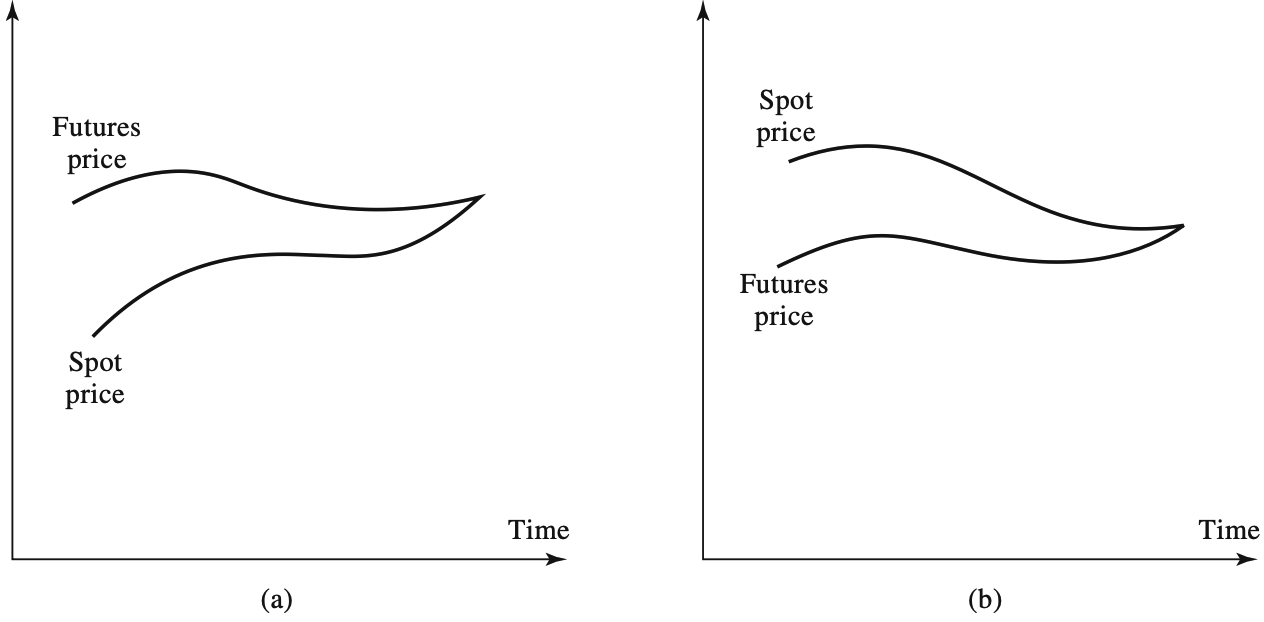
\includegraphics[scale=0.4]{derivatives/convgspotfuture}
\caption{Convergence of futures price to spot price.}
\end{figure}

Suppose futures price is above spot price during delivery period. Traders have clear arbitrage opportunity: short futures, long asset, make delivery. The futures price will then fall.\\
If futures price is below spot price during delivery period, traders will long futures, wait for delivery, and the futures price will then rise.\\

Options are traded both on exchanges and OTC.

\begin{definition} A \hlt{call option} (\hlt{put option}) gives the holder the right to sell (buy) the underlying asset by a certain date for a certain price.
\end{definition}

\begin{definition} An \hlt{American option} can be exercised at any time up to expiration date. An \hlt{European option} can only be exercised on expiration date itself.
\end{definition}

\subsubsection{Clearing House}

Margin accounts are used by exchanges to organise trading so that contract defaults are avoided. \\
Trader has to keep funds in a margin account; the amount to be deposited at the time the contract is entered into is the \hlt{initial margin}. At each of trading day, margin account is adjusted to reflect trader's P\&L (\hlt{daily settlement}, \hlt{marking to market}). Daily settlement leads to funds flowing daily between traders with long positions and traders with short positions; this daily flow of funds to reflect P\&L is the \hlt{variation margin}. Trading via brokers requires a \hlt{maintenance margin}, which is lower than initial margin; if balance in margin account falls below maintenance margin, trader receives \hlt{margin call} and is required to top up to initial margin level within short period of time, or else broker closes out the position. Trader is also entitled to withdraw any balance in margin account that is in excess of the initial margin. Brokers pay interest on balance in margin account.\\
A forward contract is settled at end of life, while futures contract is settled daily. Minimum levels for initial and maintenance margins are set by exchange clearing house. Minimum margin levels are determined by variability of the price of underlying asset, revised when necessary.\\

The clearing house acts as intermediary in futures transactions, and keep track of all daily transactions for calculating net positions of each of its members. Members must provide initial margin reflecting the total number of contracts cleared. The maintenance margin is set equal to initial margin. In determining margin requirements, the number of contracts outstanding is calculated on a net basis rather than a gross basis. Members are required to contribute to a guaranty fund, which is used in the event that a member defaults, and the member's margin is insufficient to cover losses.

\subsubsection{OTC Markets}

OTC markets use central counterparties (CCPs), which perform the same role as exchange clearing houses. Members of CCP provide both initial margin and daily variation margin, and contribute to a guaranty fund. If an OTC derivative transaction has been agreed upon between parties A and B, and CCP accepts the transaction, they become the counterparty to both A and B. CCP hence takes on credit risk of both A and B.\\
Transactions are valued daily, and there are daily variation margin payments between members.\\

For bilaterally cleared OTC, two companies enter a master agreement covering all their trades (ISDA). The agreement includes a credit support annex (CSA), requiring both parties to provide collateral. Collateral agreements in CSAs usually require transactions to be valued daily. Since 2016, regulations require both initial margin and variation margin between financial institutions.

{

\begin{definition} \hlt{Credit spread} is the difference between the interest rate and risk free rate.
\end{definition}

\hlt{(Treasury Rates)} The rates on Treasury bills and Treasury bonds. The Treasury rates of developed countries are regarded as risk-free rates, as it is assumed that there is no chance the government will default.\\

\hlt{(Overnight Rates)} Borrowing and lending overnight by financial institutions to match asset and liabilities requirements for reserves; the overnight rate is the \hlt{federal funds rate}. The weighted average of rates in brokered transactions is the \hlt{effective federal funds rate}. The Federal Reserve may intervene with its own transactions to raise or lower the rates.\\

\hlt{(Repo Rates)} Secured borrowing rates; the difference between the price at which securities are sold and then repurchased. If structured carefully, involves very little credit risk. Most common type of repo is an \hlt{overnight repo}. In longer term arrangements, \hlt{term repos} are used.\\

The terminal value of an investment $A$ invested at interest rate of $R$ per annum, compounded $m$ times per annum, is $A(1+\frac{R}{m})^{mn}$. If $m=1$, the rate is the \hlt{equivalent annual interest rate}. If continuous compounded is used, then  the terminal value at the end of a year is $Ae^{R}$.\\

The \hlt{$n$-year spot-rate} is the interest rate earned on a zero-coupon bond. The \hlt{Bond Price} is the present value of all cash flows that will be received by owner of the bond, with different spot rate for each cash flow. The \hlt{Bond Yield} is the discount rate that, when applied to all cash flows, gives a bond price equal to its market price. The \hlt{Par Yield} for a certain bond maturity is the coupon rate that causes the bond price to equal its par value.\\

\begin{definition}
\hlt{Forward Rates} are rates implied by current spot rates for periods of time in the future.
\end{definition}

Given $R_1, R_2$ the spot rates for maturities $T_1, T_2$ respectively, and $R_F$ the forward rate between $T_1$ and $T_2$, then
\begin{equation}
R_F = \frac{R_2 T_2 - R_1 T_1}{T_2 - T_1}=R_2 + (R_2 - R_1)\frac{T_1}{T_2 - T_1} \nonumber
\end{equation}
Given the spot rate $R$ for maturity $T$, the \hlt{instantaneous forward rate} for maturity of $T$ is then
\begin{equation}
R_F = R + T \frac{\partial R}{\partial T} \nonumber
\end{equation}
If $P(0,T) = e^{-RT}$ is the price of zero-coupon bond maturity at time $T$, the equation is then
\begin{equation}
R_F = -\frac{\partial}{\partial T} \ln P(0,T) \nonumber
\end{equation}

\begin{definition}
\hlt{Forward Rate Agreement (FRA)} is an agreement to exchange a predetermined rate for a reference rate that will be observed in the market at a future time.
\end{definition}

Let $R_K$ be the fixed rate, $R_F$ be the current forward rate for the reference rate, $\tau$ be the period of time to which the rates apply, $L$ be the principal in the contract.\\
For the party that receives the fix rate, the FRA has a present value of 
\begin{equation}
\tau (R_K - R_F)L \nonumber
\end{equation}
For the party that pays the fix rate, the FRA has a present value of
\begin{equation}
\tau (R_F - R_K)L \nonumber
\end{equation}

\begin{definition}
The \hlt{Duration} of a bond is a measure of how long the holder of the bond has to wait before receiving the present value of the cash payments.
\end{definition}

Let $c_i$ be cash flow at time $t_i$ ($1 \leq i \leq n$). Bond price $B$, yield $y$ (continuously compounded) are related by
\begin{equation}
B = \sum\limits_{i=1}^n c_i e^{-y t_i} \nonumber
\end{equation}
The Duration $D$ of the bond is then
\begin{equation}
D = \sum\limits_{i=1}^n t_i \left[ \frac{c_i e^{-y t_i}}{B} \right] \nonumber
\end{equation}
where the term in square brackets is ratio of present value of cash flow at $t_i$ to bond price. Duration is hence a time-weighted average of the times when payments are made.\\
The relationship between duration and yield is as follows:
\begin{align}
\Delta B &= \frac{dB}{dy} \Delta y \nonumber \\
\frac{\Delta B}{B} &= - D \Delta y \nonumber
\end{align}

If $y$ is expressed with compounding frequency of $m$ times a year, then the relationship becomes
\begin{equation}
\Delta B = - \frac{BD \Delta y}{1 + y/m} \nonumber
\end{equation}
Hence, the \hlt{modified duration} is 
\begin{equation}
D^* = \frac{D}{1 + y/m} \nonumber
\end{equation}
The duration relationship is then
\begin{equation}
\Delta B = - B D^* \Delta y \nonumber
\end{equation}

When duration is used for bond portfolios, it is assumed that the yields of all bonds will change by approximately the same amount, i.e., a parallel shift in the spot yield curve. The portfolio may still be exposed to shifts that are either large or non-parallel.\\
\hlt{Convexity} may be used to improve the relationship in the equation. Convexity is defined as
\begin{equation}
C = \frac{1}{B} \frac{d^2 B}{dy^2} \nonumber
\end{equation}
By Taylor series, we then have the relationship
\begin{equation}
\frac{\Delta B}{B} = -D \Delta y + \frac{1}{2}C(\Delta y)^2 \nonumber
\end{equation}

To determine the underlying reasons for the shape of the spot curve, theories on term structure of interest rates are referred to.\\

\hlt{(Expectations Theory)} A forward interest rate corresponding to a certain future period is equal to the expected future zero interest rate for that period.\\

\hlt{(Market Segmentation Theory)} There exists no relationship between short, medium, and long-term interest rates, as investors do not readily switch from one maturity to another.\\

\hlt{(Liquidity Preference Theory)} Investors prefer to preserve their liquidity and invest funds for short periods of time. Borrowers prefer to borrow at fixed rates for long periods of time. Hence forward rates are greater than expected future spot rates.




